Im folgenden Kapitel sollen die wichtigsten physikalischen Grundlagen für das
Verständnis der in dieser Arbeit behandelten Thematik erklärt werden. Dabei
werden die Kenntnisse über den Aufbau des Atoms, die quantisierten Lösungen der
Schrödinger- bzw. Diracgleichung, die dabei auftretenden Drehimpulskopplungen
und die daraus resultierenden Energieaufspaltungen der Atome als vorhanden
vorausgesetzt. Diesbezüglich sei auf einschlägige Lehrbücher wie
\cite{demtroeder:ex3}, \cite{demtroeder:laserspektroskopie} und \cite{saleh:grundlagen_der_photonik}
verwiesen.\\ In Kapitel \ref{sec:licht-atom-wechselwirkung} soll die Wechselwirkung von
Licht und Atom behandelt werden. Darauf aufbauend soll
in Kapitel \ref{sec:ris} die Resonanz-Ionisations-Spektroskopie,
kurz RIS, in Bezug auf die Resonanz-Ionisation von Uran-Isotopen erklärt
werden. Kapitel \ref{sec:diodenlaser} soll das Funktionsprinzip von
Halbleiterlasern und deren Rolle in diesem Projekt wiedergeben.

\section{Lich-Atom-Wechselwirkung}\label{sec:licht-atom-wechselwirkung}
Essenziell wichtig für die Resonanz-Ionisation ist das Verständnis der atomaren
Wechselwirkung mit einem elektromagnetischen Feld. Im Folgenden soll insbesondere auf die
atomaren Übergänge und deren Linienprofil eingegangen werden, da dies bei der
Atom-Spektroskopie eine wichtige Rolle spielt. Der größte Teil der dieses
Theorie-Abschnitts basiert im Wesentlichen auf den o.g. Lehrbüchern.

% $$P_{ik}=\frac{2\pi}{\hbar^2}\lvert\langle\psi_k^0\rvert\hat{\mathcal{H}}'\lvert\psi_i^0\rangle\rvert^2\delta(E_k^0-E_i^0+\hbar\omega)$$
% $$W_{ki}=\frac{\pi e^2}{3\varepsilon_0\hbar^2}\lvert\langle\psi_k\rvert\vec{r}\lvert\psi_i\rangle\rvert^2\cdot\omega_{\nu}$$
% $$B_{ki}=\frac{2}{3}\frac{\pi^2e^2}{\varepsilon_0\hbar^2}\lvert\langle\psi_k\rvert\vec{r}\lvert\psi_i\rangle\rvert^2$$
% $$\vec{M}_{ik}=e\langle\psi_i\rvert\vec{r}\lvert\psi_k\rangle$$
% $$\langle p\rangle = e\langle r\rangle = e\langle\psi_i\rvert
% r\lvert\psi_i\rangle$$
% $$\lvert\psi_k\rangle$$
% $$\bar p ^2 \rightarrow \frac{1}{2}(\lvert M_{ik}\rvert+\lvert M_{ik}\rvert)^2 =
% 2\lvert M_{ik}\rvert^2$$


\subsection{Übergangsraten}\label{subsec:uebergangsraten}
Befindet sich ein Atom in einem elektromagnetischen Feld können Absorptions- und
Emissions-Prozesse beobachtet werden. Im ersten Fall absorbiert das Atom ein
Photon einer bestimmten Mode mit der Energie $\hbar\omega_L$ aus dem elektromagnetischen Feld.
Dabei wird das Atom von einem Zustand in einen entsprechend der Photonenenergie
energetisch höher gelegenen Zustand überführt:
\begin{equation}\label{eq:uebergang}
	E_f-E_i=\hbar\omega_L
\end{equation}
Dabei ist zu beachten, dass gebundene Zustände immer quantisiert sind, also
nicht kontinuierlich im Energiespektrum verteilt sind. Analog kann ein Atom ein
Photon in das elektromagnetische Feld emittieren\footnote{Die Emission ist
auch ohne Feld möglich. Dieser Fall wird \textit{spontane Emission} genannt}.
Die Zustandsänderung des Atoms folgt dann entsprechend von einem Zustand in ein energetisch niedriger gelegenen Zustand.\par

\subsubsection{Fermis goldene Regel}\label{subsubsec:fermis_goldene_regel}
Grundlegend beschreibt \textit{Fermis goldene Regel} die
Übergangsrate von einem Zustand $\Psi_i$ (i: \textit{initial}) in einen
beliebigen Zustand $\Psi_f$ (f: \textit{final}). Diese kann halbklassisch
störungstheoretisch hergeleitet werden.  Dabei betrachtet man das externe elektromagnetische Feld als Störung
zusätzlich zum zeitunabhängigen Hamilton-Operator $\OPH_0$:
\begin{equation}\label{eq:hamilton}
	\OPH(t)=\OPH_0+\OPH'(t)
\end{equation}
mit dem Wechselwirkungsoperator
\begin{equation}\label{eq:ww}
	\begin{split}
		\OPH'(t) &= -E_0\vec{\epsilon}\cdot\OPv{d}\cos{(\vk\cdot\vr-\omega_L t)}\\
		&=
		-\OPH'\left(\mathrm{e}^{\mathrm{i}(\vk\cdot\vr-\omega_L
		t)}+\mathrm{e}^{-\mathrm{i}(\vk\cdot\vr-\omega_L t)}\right)\\
		&\text{mit}\quad
		\OPH'=\frac{1}{2}E_0\vec{\epsilon}\cdot\OPv{d}\,.
	\end{split}
\end{equation}
Hierbei ist $E_0$ die Amplitude und $\vec{\epsilon}$ der
Polarisierungsvektor des elektromagnetischen Feldes. $\OPv{d} = e\OPv{r}$ ist
der Dipoloperator. Zusätzlich kann man die Annahme machen, dass das Atom in Relation zur
Wellenlänge des Lichts sehr klein ist und es somit am Ort
des Atoms nur verschwindend geringe örtliche Änderungen der Amplitude des
elektromagnetischen Feldes erfährt ($\vk\cdot\vr\ll 1$, Atom am Ort $\vr=0$). Diese Näherung nennt man
\textit{Dipolnäherung}. Dadurch folgt für die Entwicklung des
Ortsteils der Exponentialfunktionen in erster Ordnung
$\mathrm{e}^{\pm\mathrm{i}\vk\cdot\vr}\approx1$. Nun setzt man mit der zeitabhängigen Schrödingergleichung an und entwickelt $\Psi(t)$ in die stationären Eigenzustände $\Psi_n$ des Atoms:
\begin{equation}\label{eq:sgl_stoerung_01}
	\mathrm{i}\hbar\pfrac{}{t}\ket{\Psi(t)}=\OPH(t)\ket{\Psi(t)}\,,
	\quad
	\ket{\Psi(t)}=\sum_n{c_n(t)\mathrm{e}^{-\frac{\mathrm{i}}{\hbar} E_n
	t}\ket{\Psi_n}}
\end{equation}
Führt man die Zeitableitung aus und projiziert beide Seiten der Gleichung auf
einen beliebigen Zustand $\Psi_f$, findet man
\begin{equation}\label{eq:sgl_stoerung_02}
	\dot
	c_f(t)=-\frac{\mathrm{i}}{\hbar}\sum_n{c_n(t)\mathrm{e}^{-\mathrm{i}\omega_{nf}t}\bra{\Psi_f}\OPH'(t)\ket{\Psi_n}}
	\quad\text{mit}\quad
	\omega_{nf}=\frac{E_n-E_f}{\hbar}\,.
\end{equation}
Nimmt man nun an, dass die Störung klein ist, das Atom also vornehmlich im
Ausgangs-Zustand $\Psi_i$ bleibt ($c_i(0)=1$, $c_i(t)\approx 1$, $c_{n\neq
i}\approx0$), verkürzt sich die Summe in Gl. \eqref{eq:sgl_stoerung_02}
auf einen Summanden mit $n=i\neq f$. $c_f(t)$ folgt aus zeitlicher Integration von $\dot c_f(t)$ mit
Gl. \eqref{eq:ww}:
\begin{equation}\label{eq:koeff_cf}
	\begin{split}
		c_f(t) &= \int_0^t{\dot c_f(t')\dd t'}\\
		&=
		-\frac{\mathrm{i}}{\hbar}\bra{\Psi_f}\OPH'\ket{\Psi_i}\left[\frac{\mathrm{e}^{\mathrm{i}(\omega_{fi}-\omega_L)t}-1}{\mathrm{i}(\omega_{fi}-\omega_L)}+\frac{\mathrm{e}^{\mathrm{i}(\omega_{fi}+\omega_L)t}-1}{\mathrm{i}(\omega_{fi}+\omega_L)}\right]\\
		&\text{mit}\quad
		\omega_{fi}=-\omega_{if}
	\end{split}
\end{equation}
Zu beachten ist hierbei, dass im Falle der Absorption der Nenner des zweiten
Bruchs in Gl. \eqref{eq:koeff_cf} im nahresonenten Fall
($\omega_{fi}\approx\omega_L$) in der Größenordnung $2\omega_{fi}\approx
\unit{10^{15}}{s^{-1}}$ (bei optischen Übergängen) liegt. Somit wird der
zweite Bruch verschwindend gering gegenüber dem ersten und kann vernachlässigt
werden. Im Falle der Emission betrachtet man Übergänge vom energetisch höheren
Niveau zum energetisch niedrigeren Niveau. Dabei gilt
($\omega_{if}\approx\omega_L$), wodurch der erste Bruch vernachlässigt werden
kann. Im Folgenden wird allerdings exemplarisch die Absorption betrachtet.\\
Für die Übergangswahrscheinlichkeit ergibt sich
\begin{equation}\label{eq:uebergangs_wkt}
	\begin{split}
		P_{i\to f}(t,\Delta\omega) &= \abs{c_f(t)}^2\\
		& =
		\frac{1}{\hbar^2}\abs{\bra{\Psi_f}\OPH'\ket{\Psi_i}}^2\cdot\frac{\sin^2{\left(\frac{\Delta\omega}{2}t\right)}}{\left(\frac{\Delta\omega}{2}\right)^2}\\
		&\text{mit}\quad
		\Delta\omega=\omega_L-\omega_{fi}\,.
	\end{split}
\end{equation}
Für die totale Übergangswahrscheinlichkeit gilt dann mit Gl.
\eqref{eq:uebergangs_wkt}
\begin{equation}\label{eq:uebergangs_wkt_total}
	\begin{split}
		P_{i\to f}(t)
		&= \int{P_{i\to f}(t,\Delta\omega)\rho(E_f)}\dd E_f\\
		&\approx \rho(E_f)\int{P_{i\to f}(t,\Delta\omega)}\dd E_f\\
		&= \hbar\rho(E_f)\int_{-\infty}^{\infty}{P_{i\to
		f}(t,\Delta\omega)}\dd(\Delta\omega)\\
		&= \frac{2\pi t}{\hbar}\rho(E_f)\abs{\bra{\Psi_f}\OPH'\ket{\Psi_i}}^2\,.
	\end{split}
\end{equation}
Hierbei wurde die Energieniveaudichte $\rho(E_f)=\fracd{n}{E_f}$ eingeführt. Sie
beschreibt die Verteilung der Energieniveaus der Endzustände $E_f$. Mit
der Annahme, dass sich $\rho(E_f)$ gegenüber $P_{i\to f}(t,\Delta\omega)$ nur langsam ändert, kann $\rho(E_f)$ in Gl. \eqref{eq:uebergangs_wkt_total}
als hinreichend konstant angenommen und aus dem Integral gezogen werden.
Weiterhin wurde die Substitution $\dd E_f=\hbar\dd(\Delta\omega)$ vorgenommen. Für die
totale Übergangsrate folgt dann mit Gl. \eqref{eq:uebergangs_wkt_total}
für genügend große Zeiten ($t\gg\frac{1}{\omega_{fi}}$) Fermis goldene Regel:
\begin{equation}\label{eq:uebergangs_rate_total}
	\boxed{
		\begin{split}
			\Gamma_{i\to f}
			&= \lim_{t\to\infty}{\left(\fracd{}{t}{P_{i\to f}(t)}\right)}\\
			&= \frac{2\pi}{\hbar}\rho(E_f)\abs{\bra{\Psi_f}\OPH'\ket{\Psi_i}}^2
		\end{split}
	}
\end{equation}

$\bra{\Psi_f}\OPH'\ket{\Psi_i} =
\frac{1}{2}E_0\vec{\epsilon}\cdot e\bra{\Psi_f}\OPv{r}\ket{\Psi_i}$ enthält
das sog. \textit{Dipolmatrixelement} $e\bra{\Psi_f}\OPv{r}\ket{\Psi_i}$ für die Zustände
$\Psi_i$ und $\Psi_f$. Es gibt an, ob ein Übergang im Rahmen der Dipolnäherung
erlaubt oder verboten ist. Dazu sei auf Kapitel \ref{subsec:auswahlregeln} verwiesen.

\subsubsection{Einsteinkoeffizienten}\label{subsubsec:einsteinkoeffizienten}
Bisher wurden Absorption und Emission nur allgemein behandelt. Bei der Emission
muss man allerdings zwischen der \textit{induzierten} und der \textit{spontanen
Emission} unterscheiden. Die induzierte Emission findet nur mit vorhandenem
elektromagnetischen Feld statt. Es wird ein Photon der entsprechenden Mode aus
dem elektromagnetischen Feld benutzt, um eine Emission zu induzieren und ein
weiteres Photon in das Feld zu emittieren. Bei der spontanen Emission hingegen
fällt das Atom spontan in einen energetisch niedrigeren Zustand und ein
Photon der entsprechenden Mode wird emittiert (auch ohne Feld).\\ In einem
elektromagnetischen Feld mit spektraler Energiedichte $w(\nu)=n(\nu)h\nu$, bei der $n(\nu)=\pfrac{n}{\nu}$ die spektrale Photonendichte ist, sind im stationären Gleichgewicht die
Besetzungszahlen $N_i$ des höheren Niveaus und $N_k$ des niedrigeren Niveaus zeitlich konstant. In der Ratengleichung
\begin{equation}\label{eq:raten_gleichung}
	A_{ik}N_i+B_{ik}w(\nu)N_i=B_{ki}w(\nu)N_k
\end{equation}
sind hierfür Emissionsraten und Absorptionsraten gleichgesetzt.
Die beiden Größen

\begin{subequations}\label{eq:einsteinkoeff_wkten}
	\begin{equation}\label{eq:einsteinkoeff_wkten_ik}
		W_{ki}=B_{ki}w(\nu)
	\end{equation}
	\begin{equation}\label{eq:einsteinkoeff_wkten_ki}
		W_{ik}=B_{ik}w(\nu)
	\end{equation}	
\end{subequations}
geben die Wahrscheinlichkeiten für die Absorption (a) und die induzierte
Emission (b) an, wobei $B_{ki}$ bzw. $B_{ki}$ die jeweiligen sog.
\textit{Einsteinkoeffizienten} sind. $A_{ik}$ ist der Einsteinkoeffizient für
die spontane Emission. Zeichnung \ref{fig:einstein_koeffizienten}
veranschaulicht dies.\\
\begin{figure}[h]
	\centering
	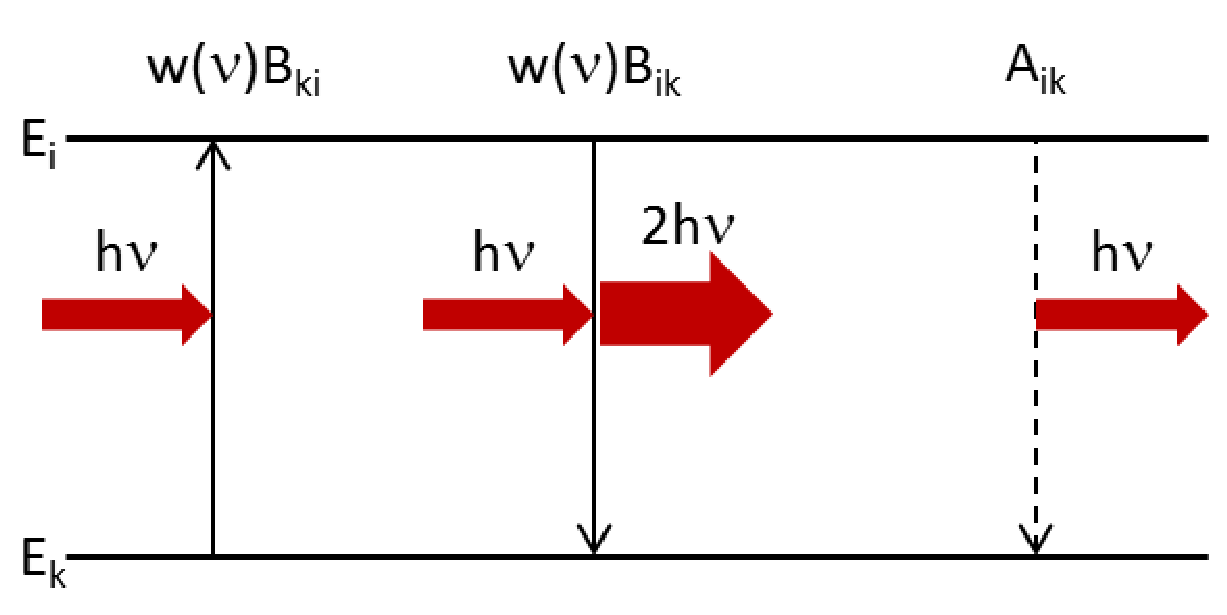
\includegraphics[width=10cm]{gfx/einstein_koeffizienten.eps}
	\caption{zwei Energieniveaus eines Atoms mit Absorption,
	induzierte Emission und spontane Emission (von links nach
	rechts)}\label{fig:einstein_koeffizienten}
\end{figure}

Im thermischen Gleichgewicht sind die Besetzungszahlen
boltzmann-verteilt \cite{demtroeder:ex3}:
\begin{equation}\label{eq:boltzmann_verteilung}
	\begin{split}
		\frac{N_i}{N_k}&=\frac{g_i}{g_k}\mathrm{e}^{-\frac{(E_i-E_k)}{kT}}\\[0.2cm]
		&=\frac{g_i}{g_k}\mathrm{e}^{-\frac{h\nu}{kT}}\,.
	\end{split}	
\end{equation}
$g_i$ und $g_k$ sind die Entartungsgrade ($2J+1$) der jeweiligen Niveaus und
sind damit eine statistische Gewichtung der Niveaus.
Kombiniert man \eqref{eq:raten_gleichung} und \eqref{eq:boltzmann_verteilung}
und löst nach $w(\nu)$ auf, findet man
\begin{equation}\label{eq:spektrale_energiedichte_1}
	w(\nu)=\frac{\nicefrac{A_{ik}}{B_{ik}}}{\left(\nicefrac{g_i}{g_k}\right)\left(\nicefrac{B_{ik}}{B_{ki}}\right)\left(\mathrm{e}^\frac{h\nu}{kT}-1\right)}\,.
\end{equation}
Führt man einen Koeffizientenvergleicht mit der spektralen
Energiedichte eines thermischen Strahlungsfeldes \cite{demtroeder:ex3}
\begin{equation}\label{eq:spektrale_energiedichte_2}
	w(\nu)=\frac{8\pi h\nu^3}{c^3}\frac{1}{\mathrm{e}^\frac{h\nu}{kT}-1}
\end{equation}
durch, findet man folgende Beziehungen der Einsteinkoeffizienten:
\begin{subequations}\label{eq:einsteinkoeff_relationen}
	\begin{equation}\label{eq:einsteinkoeff_relationen_1}
		B_{ik}=\frac{g_k}{g_i}B_{ki}
	\end{equation}
	\begin{equation}\label{eq:einsteinkoeff_relationen_2}
		A_{ik}=\frac{8\pi h\nu^3}{c^3}B_{ik}\,.
	\end{equation}
\end{subequations}
%**blabla_01
blabla01
%blabla_01**
\par
Im Folgenden sollen die Einsteinkoeffizienten berechnet werden.
Zur Berechnung des Koeffizienten der spontanen Emissionswahrscheinlichkeit
betrachtet man das Atom als Hertzschen Dipol, der radial isotrop abstrahlt. Die
zeitlich mittlere abgestrahlte Leistung von $N_i$ Atomen
\cite{demtroeder:ex3} ist
\begin{equation}\label{eq:abgestrahlte_leistung_01}
	\mean{P}_t = \frac{1}{3}N_i\frac{\omega_{ik}^4}{\pi\epsilon_0
	c^3}\abs{\OPv{d}_{ik}}^2
\end{equation}
mit dem bereits erwähnte Dipolmatrixelement
$\OPv{d}_{ik}=e\bra{\Psi_i}\OPv{r}\ket{\Psi_k}$. Definiert man den
Einsteinkoeffizienten der spontanen Emission $A_{ik}$ als Wahrscheinlichkeit pro
Sekunde, dass ein Atom spontan von $\ket{\Psi_i}$ in $\ket{\Psi_k}$ übergeht,
ist Gl. \eqref{eq:abgestrahlte_leistung_01} identisch mit
\begin{equation}\label{eq:abgestrahlte_leistung_02}
	\mean{P}_t=N_iA_{ik}h\nu_{ik}\,.
\end{equation}
Daraus folgt
\begin{equation}\label{eq:abgestrahlte_leistung_02}
	\boxed{
		A_{ik}=\frac{2}{3}\frac{\omega_{ik}^3}{\epsilon_0c^3h}\abs{\OPv{d}_{ik}}^2
	}\,.
\end{equation}
Um die Einsteinkoeffizienten für die Absorption und induzierte Emission
auszurechnen, setzt man mit der Absorptionswahrscheinlichkeit pro Sekunde an
(oben hergeleitete Fermis goldene Regel \eqref{eq:uebergangs_rate_total}):
\begin{equation}\label{eq:w_ki_01}
	W_{k\to i}
	= \frac{2\pi}{\hbar}\rho(E_k)\abs{\bra{\Psi_i}\OPH'\ket{\Psi_k}}^2
\end{equation}
Die Energieniveadichte lässt sich schreiben als
$\rho(E)=\pfrac{n}{E}=\frac{1}{h}\pfrac{n}{\nu}$.
Das zeitliche Mittel der spektralen Energiedichte des elektromagnetischen Feldes
ist $\mean{w(\nu)}_t=\pfrac{n}{\nu}\frac{1}{2}\epsilon_0 E^2_0$. Damit lässt
sich die Energieniveaudichte in Relation zur spektralen Energiedichte schreiben:
\begin{equation}\label{eq:energieniveaudichte_spektrale_energiedichte}
	\rho(E)=\frac{2\mean{w(\nu)}_t}{\epsilon_0 E_0^2h}\,.
\end{equation}
Setzt man Gl. \eqref{eq:energieniveaudichte_spektrale_energiedichte} in
Gl. \eqref{eq:w_ki_01} ein und schreibt das Matrixelement
zu $\bra{\Psi_i}\OPH'\ket{\Psi_k} =
\frac{1}{2}E_0\vec{\epsilon}\cdot\OPv{d}_{ki}$ um, erhält
man unter der Annahme eines isotropen Strahlungsfeldes
($\mean{\abs{\vec{\epsilon}\cdot\vr}^2} = \frac{1}{3}\abs{\vr}^2$)
\begin{equation}\label{eq:w_ki_02}
	W_{ki}
	= \frac{2\pi^2}{3h^2\epsilon_0}\abs{\OPv{d}_{ki}}^2\mean{w(\nu)}_t\,.
\end{equation}
Ein Vergleich mit Gl. \eqref{eq:einsteinkoeff_wkten_ik} liefert
\begin{equation}\label{eq:w_ki_02}
	\boxed{
		B_{ki} = \frac{2\pi^2}{3h^2\epsilon_0}\abs{\OPv{d}_{ki}}^2
	}\,.
\end{equation}
Das Ergebnis ist konsistent mit den in Gl.
\eqref{eq:einsteinkoeff_relationen} beschriebenen Relationen der
Einsteinkoeffizienten.

\subsection{Auswahlregeln}\label{subsec:auswahlregeln}
Damit ein Übergang im Rahmen der Dipolnäherung \textit{erlaubt} ist, darf das
Dipolmatrixelement nicht verschwinden:
\begin{equation}\label{eq:dipolmatrixelement}
	e\bra{\Psi_i}\OPv{r}\ket{\Psi_k}\neq0
\end{equation}
\textit{Verbotene} Übergänge können allerdings bei Betrachtung von
Matrixelementen höherer Ordnung sehr wohl erlaubt sein, sind jedoch sehr stark
unterdrückt. Welche Übergänge nun erlaubt und welche verboten sind, hängt von
der Konfiguration bzw. den Quantenzahlen der beiden Zustände ab:
\begin{equation}\label{eq:dipolmatrixelement_quantenzahlen}
	\bra{n_i,L_i,S_i,m_{L_i}, m_{S_i}}\OPv{r}\ket{n_k,L_k,S_k,m_{L_k}, m_{S_k}}
\end{equation}
Vorrausgesetzt wird, dass die l-l- und s-s-Kopplungen der einzelnen Elektronen
untereinander im Atom stark gegenüber der l-s-Kopplung sind (LS-Kopplung stark).
Dies ist bei schweren Atom nicht mehr gegeben. Dort dominieren die einzelnen
l-s-Kopplungen. (jj-Kopplung stark)\\
Da im Gesamtsystem die Drehimpulserhaltung
gelten muss, gilt für $\Delta L =\pm1$. Bei Absorption eines Photons wird aus dem elektromagnetischen Feld ein Photon (Boson, Spin 1) mit dem Drehimpuls vom Betrag 1 entnommen, was durch den Drehimpuls des Atoms wieder kompensiert werden muss. Analog verhält es sich bei der Emission. $\Delta L =\pm1$ kann auch mit die erforderliche unterschiedlichen Parität der Zustände begründet werden ($\OPP\ket{\psi}=(-1)^L\ket{\psi}$). Der
Ortsoperator hat ungerade Parität. Insgesamt muss sich bei der Berechnung des Matrixelements eine gerade Funktion ergeben, damit dieses von 0
verschieden ist. Dies ist nur mit unterschiedlicher Parität beider Zustände
möglich $(-1)^{L_i}\neq(-1)^{L_k}$, was für
ungerade $\Delta L$ gilt. Die Begrenzung auf $\pm1$ ist durch den Spin 1 des
Photons begründet. Die Änderung der Projektion des Drehimpulses auf die Quantisierungsachse ist mit der
Polarisation des Photons verknüpft. Bei der Absorption von zirkular
polarisiertem Licht, das sich senkrecht zur Quantisierungsachse ausbreitet, ist
der Photonen-Drehimpuls +1 für $\sigma^+$-Polarisation und -1 für
$\sigma^-$-Polarisation. Linearpolarisiertes Licht ist eine Kombination aus
$\sigma^+$- und $\sigma^-$-polarisiertem Licht. Die Projektion des Drehimpulses
ändert sich in diesem Fall nicht. Es gilt also $\Delta m_L = 0, \pm1$.
Die Spinwellenfunktion wird bei Dipolübergängen nicht beeinflusst. Daher gilt
$\Delta S=0$. Weiterhin gilt für $\vJ=\vL+\vS$ die Änderung $\Delta J=0,\pm1$.
$\Delta J=0$ rührt daher, dass die Änderung $\Delta L=\pm1$ durch die entgegengesetzte
Änderung $\Delta m_S=\mp1$ kompensiert wird, was allerdings für
$J=0\leftrightarrow0$ nicht gelten kann. Für die Kopplung an den Kernspin gilt
analoge Überlegung: $\Delta F = 0, \pm1$ außer bei $F=0\leftrightarrow0$. In
Tabelle \ref{tab:auswahlregeln} sind alle Auswahlregeln noch einmal
aufgelistet.

\begin{table}
	\begin{tabular}{p{0.15\textwidth}p{0.37\textwidth}p{0.37\textwidth}}

		\toprule
		Regel & Ursache & Einschränkungen \\
		\midrule[1px]
		\hline
		$\Delta L = \pm1$ & Parität / Gesamtdrehimpulserhaltung & in LS-Kopplung \\
		$\Delta m_L = 0, \pm1$ & Polarisation / Drehimpuls des Photons & \\
		$\Delta S = 0$ & em. Feld koppelt nicht an Spin & gilt nicht mehr für schwere
		Atome mit jj-Kopplung \\
		$\Delta m_S = 0, \pm1$ & Spinorientierung & \\
		$\Delta J = 0, \pm1$ & Spin-Drehimpuls-Kombinationen & mit Ausnahme von
		$J=0\leftrightarrow0$
		\\
		$\Delta F = 0, \pm1$ & Kernspin-J-Kombinationen & mit Ausnahme von
		$F=0\leftrightarrow0$
		\\
		\bottomrule[1px]
	\end{tabular}
	\caption{Auswahlregeln, deren Ursache und Einschränkungen}
	\label{tab:auswahlregeln}
\end{table}



\subsection{Linienprofil}\label{sec:linienprofil}

\section{Resonanz-Ionisations-Spektroskopie}\label{sec:ris}

\section{Diodenlaser in der RIS}\label{sec:diodenlaser}
%\cite{chow:semiconductor-laser}